\documentclass[a4paper]{article}

\usepackage{amsfonts}
\usepackage{amsmath}
\usepackage{graphicx}
\usepackage{bbold}

\title{Theoretical background for cubic B-spline evaluation}
\author{Sven Proppert}

\begin{document}

\maketitle

\begin{figure}%
\centering
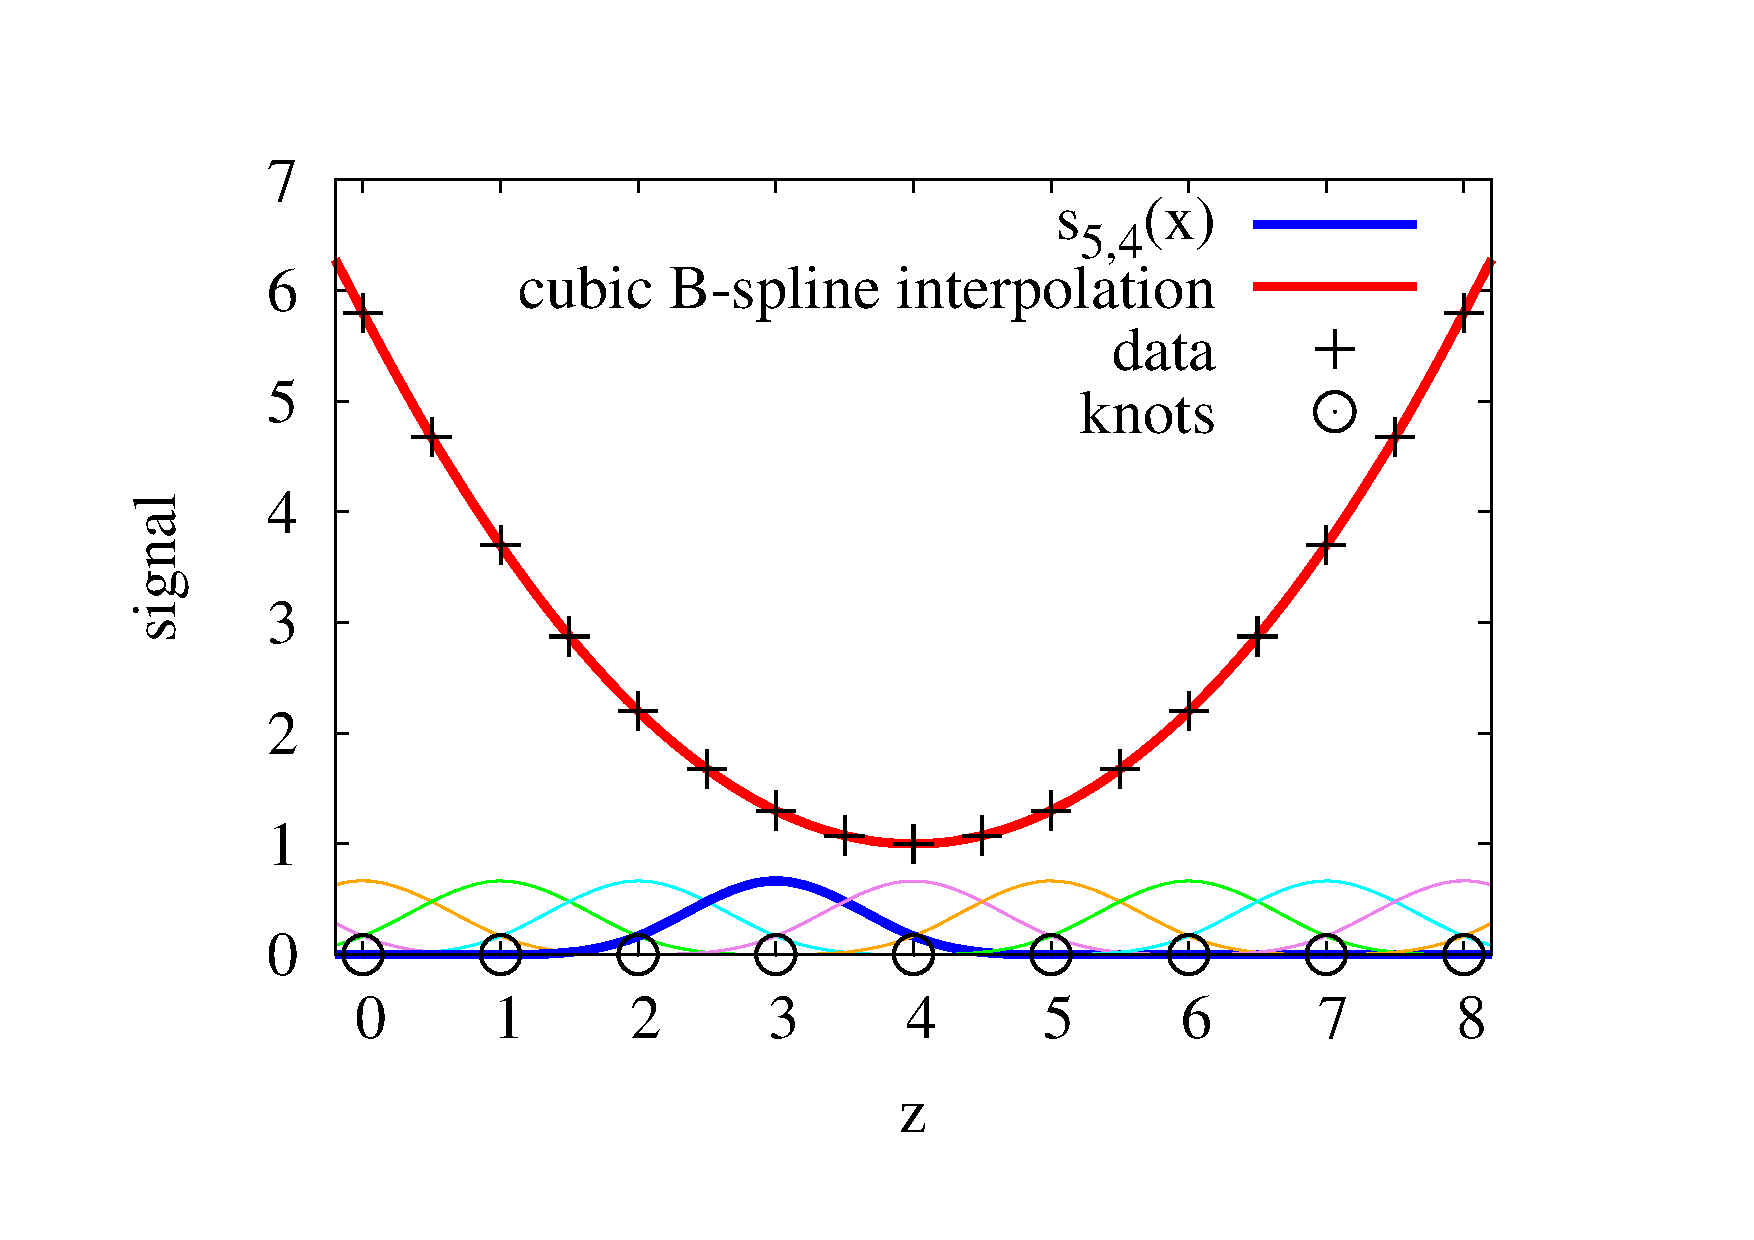
\includegraphics[width=0.7\columnwidth]{spline-theory-example.pdf}%
\caption{This diagram (arbitrary units) aims to visualise exemplarily how to handle data with cubic B-spline interpolation. The black crosses represent seventeen given data points while the rainbow-colored pseudo-Gaussians at the bottom of the diagram are plots of the B-spline basis functions $s_{i,4}(x)$ $(i=0,1,\hdots ,11)$ with the $n=9$ knots indicated by black circles. Evaluation of eq.\ref{eq:lsf} leads to amplitude factors for each basis function. The superposition with given amplitudes results in the interpolation represented by the red parabola.}%
\label{fig:ex}%
\end{figure}

\section{Definition of B-spline basis functions}
Consider a given dataset of $m$ points $y_0(x_0)\, , \,y_1(x_1)\, , \, \hdots \, , \, y_m(x_m)$ on an interval $[L_1:L_2]$ (black crosses in fig.\ref{fig:ex}). In order to perform the interpolation, first that interval is split into segments represented by $n$ equidistant knots $t_{i}$ $\left(i=0,1,\hdots ,n-1\right)$ marked as black circles.
As implemented in the GNU Scientific Library for B-spline-interpolation, the $n+2$ basis functions $s_{i}(x)$ of order $k$ are segmentwise recursively defined following equations \ref{eq:bi1} and \ref{eq:bik}. For cubic B-splines, $k$ goes from 1 to 4.

\begin{equation}
s_{i,1}(x) = \left\{\begin{array}{ll}
                  1\;         &:\, t_i \leq x < t_{i+1}\\
                  0\;                &:\, else
                  \end{array}\right.
\label{eq:bi1}
\end{equation}

\begin{equation}
s_{i,k}(x) = \frac{x - t_i}{t_{i+k-1} - t_i} s_{i,k-1}(x)+ \frac{t_{i+k} - x}{t_{i+k} - t_{i+1}} s_{i+1,k-1}(x)
\label{eq:bik}
\end{equation}\\

\section{Interpolation and least squares fitting (LSF) as implemeted in rapi\textit{d}STORM}
The interpolation to the dataset is computed as in eq.\ref{eq:lgs} and represents a set of linear equations with $\vec{y}=\left(y_0(x_0)\, , \,y_1(x_1)\, , \, \hdots \, , \, y_m(x_m)\right)$ and $\vec{c}=\left(c_0\, , \,c_1\, , \, \hdots \, ,\, c_{n} \, , \, c_{n+1}\, , \,c_{n+2}\right)$. Matrix notation (eq.\ref{eq:matrix}) indicates, that $S$ is of diagonal form.

\begin{align}
y_m(x_m) &= \sum_i s_{i,k}(x_m) c_i\nonumber\\
\vec{y} &= S \cdot \vec{c}\label{eq:lgs}
\end{align}

\scriptsize
\begin{equation}
\left(\begin{array}{c}
y_0\\
y_1\\
\vdots\\
y_{m-3}\\
y_{m-2}\\
y_{m-1}\\
y_{m}
\end{array}\right)= \left(\begin{array}{ccccccc}
        s_{0}(x_{0}) &s_{1}(x_{0}) &s_{2}(x_{0})         &0                                                 &0                                                 &\cdots                  &0\\
        s_{0}(x_{1}) &s_{1}(x_{1}) &s_{2}(x_{1})         &s_{3}(x_{1})         &0                                                 &\cdots                  &0\\
        0                                         &s_{1}(x_{2}) &s_{2}(x_{2})         &s_{3}(x_{2})         &0                                                 &\cdots                 &0\\
        0                                         &s_{1}(x_{3}) &s_{2}(x_{3})         &s_{3}(x_{3})         &s_{4}(x_{3})         &\cdots                 &0\\
        \vdots                        &\vdots                                                &\ddots                                &\ddots                                &\ddots                                &\ddots                &\vdots\\        
        0                                                &0                                                &0                                                        &s_{n-1}(x_{m-1})                                                        &s_{n}(x_{m-1})                &s_{n+1}(x_{m-1})                                        &s_{n+2}(x_{m-1})\\
        0                                                &0                                                &0                                                        &0                                                        &s_{n}(x_{m})                &s_{n+1}(x_{m})                                        &s_{n+2}(x_{m})
\end{array}\right)\cdot \left(\begin{array}{c}
c_0\\
c_1\\
\vdots\\
c_{n-1}\\
c_n\\
c_{n+1}\\
c_{n+2}
\end{array}\right)
\normalsize\label{eq:matrix}                                        %%auch wenn mir mein compiler ne warung rausgibt, dass normalsize im math mode unzul�ssig ist, funktioniert's, dass die formel-nummer nicht zu klein angezeigt wird... wenn wem was sch�neres einf�llt bitte her damit
\end{equation}
%%        0                                                &0                                                &0                                                        &0                                                        &s_{n-3}(x_{m-2})                                                        &s_{n-2}(x_{m-2})                &s_{n-1}(x_{m-2})                                        &0\\%%$$

\normalsize
In equation \ref{eq:lgs} the vector $\vec{c}$ is unknown and is object to least squares fitting, which is performed following eq.\ref{eq:lsf}.
\begin{equation}
\vec{c}=(S^{T}\cdot S)^{-1}\cdot S^{T} \cdot \vec{y}
\label{eq:lsf}
\end{equation}

\subsection{Derivation of the formula for LSF (eq.\ref{eq:lsf})}
The fit residuals are defined as: $\vec{r}(\vec{c})=\vec{y}-S\cdot\vec{c}$ with the $i$-th component of r being: $r_i(c_j)=y_i - \sum\limits_j S_{ij} \cdot c_j$. The least squares fitting criteria is fulfilled when
\begin{equation}
\left|\vec{r}(\vec{c})^2\right|=\mathrm{min}\Leftrightarrow\frac{\partial \vec{r}(\vec{c})^2}{\partial \vec{c}}=0\;\;\;\;\;\;.
\label{eq:lscrit}
\end{equation}
Evaluation of the right side of eq.\ref{eq:lscrit} for $r_i$ gives
\begin{align}
0 &= \sum\limits_i \frac{\partial \left(r_i(c_j)^2\right)}{\partial c_j} = \sum\limits_i \frac{\partial r_i(c_j)}{\partial c_j}\cdot 2r_i(c_j)\nonumber \\
&= \sum\limits_i -S_{ij}\cdot 2r_i(c_j) =\sum\limits_i S_{ij} \cdot \left[y_i - \sum\limits_k S_{ik} \cdot c_k\right]\nonumber\\
&=\sum\limits_i S_{ij}\cdot y_i\,-\, \sum\limits_i S_{ij}\cdot\sum\limits_k S_{ik} \cdot c_k \nonumber
%%\label{eq:berabla}
\end{align}

\begin{align}
\sum\limits_i S_{ij}\cdot y_j &= \sum\limits_k\left[\sum\limits_i S_{ij} \cdot S_{ik}\right] \cdot c_k \nonumber \\
\sum\limits_i S^{T}_{ji}\cdot y_i&= \sum\limits_k \left[\sum\limits_i S^T_{ji} \cdot S_{ik}\right] \cdot c_k \nonumber \\
&= \sum\limits_k \left(S^T\cdot S\right)_{jk}\cdot c_k \nonumber \\
\left(S^T\cdot\vec{y}\right)_j&= \left[\left(S^T\cdot S\right)\vec{c}\right]_j
\label{eq:berabl}
\end{align}
which, rewritten in vector notation leads to the form of eq.\ref{eq:lsf}:
\begin{align}
S^T \vec{y} &=\left(S^T\cdot S\right)\vec{c}\nonumber\\
\Leftrightarrow \left(S^T\cdot S\right)^{-1} S^T \vec{y} &= \mathbb{1}\vec{c}\;\;\;\;\;\;.
\label{eq:qed}
\end{align}

\end{document}